\chapter{APT Detection Solutions}
\label{chap:apt\_solutions}

\section{Introduction}

Advanced Persistent Threats (APTs) represent one of the most complex challenges in the modern cybersecurity landscape. Characterized by their stealth, longevity, and multi-stage execution, APTs often evade traditional signature-based detection mechanisms. Consequently, the research community has shifted focus towards behavioral analysis and artificial intelligence (AI) to identify these sophisticated attacks. This chapter provides a detailed classification and description of existing APT detection solutions, synthesizing the state-of-the-art based on recent literature, particularly the extensive survey by Ankalaki et al. \cite{ankalaki2025cyber}. We then conduct a dedicated study of the datasets most relevant to APT detection research, examining both their characteristics and the AI/ML works that have used them. Finally, we present our proposed framework, which integrates Generative AI, Reinforcement Learning, and Graph Neural Networks to address the identified gaps in early detection and automated response.

---

\section{Classification of Solutions}

Based on the comprehensive analysis provided by Ankalaki et al. \cite{ankalaki2025cyber}, detection solutions for cyber-attacks and APTs can be broadly categorized based on the underlying algorithmic evolution and learning paradigms. The classification progresses from traditional statistical methods to advanced generative models.

\subsection{Traditional Machine Learning (ML) Approaches}

Traditional ML approaches constitute the foundational layer of intelligent detection. As highlighted in \cite{ankalaki2025cyber}, these are further divided based on the availability of labeled data:

\begin{itemize}
\item \textbf{Supervised Learning:} These algorithms require fully labeled datasets (benign vs. malicious). They are widely used for malware classification and detecting known intrusion patterns but struggle with zero-day attacks.
\item \textbf{Unsupervised Learning:} These methods operate on unlabeled data, aiming to discover hidden structures or anomalies. In the context of APTs, unsupervised learning is critical for identifying deviations from "normal" network baselines without prior knowledge of the attack signature.
\item \textbf{Semi-supervised Learning:} A hybrid approach that utilizes a small amount of labeled data alongside a large volume of unlabeled data, addressing the scarcity of annotated APT datasets.
\end{itemize}

\subsection{Deep Learning (DL) Approaches}

Deep Learning represents a subset of ML that utilizes multi-layered neural networks to learn hierarchical representations of data. Ankalaki et al. \cite{ankalaki2025cyber} emphasize that DL models outperform traditional ML in handling unstructured high-dimensional data, such as raw network traffic bytes or system log sequences. Key architectures in this category include Convolutional Neural Networks (CNNs) and Recurrent Neural Networks (RNNs).

\subsection{Generative Artificial Intelligence (GenAI) Approaches}

The most recent evolution in detection strategies involves Generative AI. Unlike discriminative models that separate classes, generative models (such as VAEs and GANs) learn the underlying distribution of the data to generate new instances. According to \cite{ankalaki2025cyber}, GenAI is revolutionizing cybersecurity by enabling:

\begin{enumerate}
\item \textbf{Advanced Anomaly Detection:} By learning the exact distribution of benign traffic, any deviation — even subtle — can be flagged with high precision.
\item \textbf{Data Augmentation:} Generating synthetic attack data to train models, addressing the critical lack of real-world APT samples.
\item \textbf{Adversarial Defense:} Simulating attacks to harden defense systems.
\end{enumerate}

---

\section{Description of Solutions}

This section details the technical mechanisms of the algorithms identified in the classification, evaluating their specific application to APT detection as discussed in \cite{ankalaki2025cyber}.

\subsection{Machine Learning Solutions}

\textbf{Support Vector Machines (SVM)}

SVM is a supervised learning algorithm that constructs a hyperplane or set of hyperplanes in a high-dimensional space to separate classes (e.g., Normal vs. Attack):

\[f(x) = \text{sign}\!\left(\sum\_{i=1}^{n} \alpha\_i y\_i K(x\_i, x) + b\right)\]

As noted in \cite{ankalaki2025cyber}, SVMs are effective for high-dimensional data but entail high computational costs during the training phase, making them less suitable for real-time processing of massive network flows.

\textbf{Random Forest (RF) and Decision Trees}

Decision Trees (DT) provide high interpretability by splitting data based on feature values. Random Forest (RF) improves upon DT by aggregating multiple trees (bagging) to reduce overfitting. Ankalaki et al. \cite{ankalaki2025cyber} report that RF achieves high accuracy (often exceeding 99\%) in detecting specific attack types like DDoS and Botnets within IoT environments, making it a robust baseline for APT stage detection.

\textbf{Naïve Bayes (NB)}

Based on Bayes' theorem with an assumption of feature independence, NB is computationally efficient. While it lacks the nuance to detect complex, correlated APT behaviors, it serves as a fast filter for initial traffic classification \cite{ankalaki2025cyber}.

\textbf{Table 3.1 — Performance Analysis of State-of-the-Art ML Approaches for Cyber-Attack Prediction \cite{ankalaki2025cyber}}

| Dataset | Model | Accuracy (\%) | Precision | Recall | F1-Measure |
|---|---|---|---|---|---|
| AWID | AdaBoost | 92.20 | 0.850 | 0.922 | 0.885 |
| AWID | Naïve Bayes | 89.43 | 0.891 | 0.894 | 0.877 |
| AWID | Random Forest (RF) | 95.58 | 0.958 | 0.956 | 0.941 |
| Modern DDoS | MLP | 98.63 | 0.986 | 0.986 | 0.986 |
| Modern DDoS | Random Forest (RF) | 98.02 | 0.980 | 0.980 | 0.980 |
| Modern DDoS | Naïve Bayes | 96.91 | 0.969 | 0.969 | 0.969 |
| CICIDS2017 | KNN | 96.00 | 0.960 | 0.960 | 0.960 |
| CICIDS2017 | Random Forest (RF) | 98.00 | 0.980 | 0.970 | 0.970 |
| CICIDS2017 | ID3 | 98.00 | 0.980 | 0.980 | 0.980 |
| CICIDS2017 | Naïve Bayes | 75.00 | 0.880 | 0.040 | 0.040 |
| HIKARI-2021 | KNN | 98.00 | 0.860 | 0.900 | 0.880 |
| HIKARI-2021 | MLP | 99.00 | 0.990 | 0.990 | 0.990 |
| HIKARI-2021 | SVM | 99.00 | 0.990 | 0.980 | 0.990 |
| HIKARI-2021 | Random Forest (RF) | 99.00 | 0.990 | 0.990 | 0.990 |
| CICAndMal2017 | Random Forest (RF) | 85.00 | 0.850 | 0.880 | 0.860 |
| CICAndMal2017 | KNN | 85.00 | 0.850 | 0.880 | 0.860 |
| CICAndMal2017 | Decision Tree (DT) | 85.00 | 0.850 | 0.880 | 0.860 |
| MQTT-IoT-IDS2020 | Logistic Regression | 99.44 | 0.990 | 0.990 | 0.990 |
| MQTT-IoT-IDS2020 | KNN | 99.90 | 0.990 | 0.990 | 0.990 |
| MQTT-IoT-IDS2020 | Decision Tree (DT) | 99.95 | 0.995 | 0.995 | 0.995 |
| MQTT-IoT-IDS2020 | Random Forest (RF) | 99.97 | 0.997 | 0.997 | 0.997 |

\subsection{Deep Learning Solutions}

\textbf{Convolutional Neural Networks (CNN)}

Originally designed for image processing, CNNs are applied to cybersecurity by treating network traffic as images or matrices. They excel at extracting spatial features (local patterns) from traffic payloads. \cite{ankalaki2025cyber} highlights their utility in malware classification where binary executables are visualized as grayscale images.

\textbf{Recurrent Neural Networks (RNN) and LSTM}

Given that APTs are temporal, multi-stage attacks, standard feed-forward networks often fail to capture the sequence of events. RNNs address this by maintaining a "memory" of previous inputs. Specifically, Long Short-Term Memory (LSTM) networks are crucial for APT detection because they solve the vanishing gradient problem, allowing the model to learn long-term dependencies:

\[f\_t = \sigma(W\_f \cdot [h\_{t-1}, x\_t] + b\_f)\]

This capability allows LSTMs to correlate a "Reconnaissance" event (Stage 1) with an "Exfiltration" event (Stage 7) that occurs days or weeks later \cite{ankalaki2025cyber}.

\textbf{Table 3.2 — Performance Analysis of State-of-the-Art DL Approaches for Cyber-Attack Prediction \cite{ankalaki2025cyber}}

| Dataset | Model | Accuracy (\%) | Precision | Recall | F1-Measure |
|---|---|---|---|---|---|
| NSL-KDD | FCN | 89.40 | 0.877 | 0.946 | 0.910 |
| PDF Documents | MLP | 97.50 | 0.991 | 0.998 | 0.994 |
| UGR16 | Adversarial Autoencoder (AAE) | 96.70 | 0.931 | 0.965 | 0.948 |
| TON-IoT | LSTM | 97.00 | 0.970 | 0.960 | 0.970 |
| TON-IoT | CNN | 99.00 | 0.980 | 0.990 | 0.990 |
| Bot-IoT | LSTM | 98.05 | 0.999 | 0.980 | 0.990 |
| Bot-IoT | RNN | 97.90 | 0.999 | 0.979 | 0.989 |
| SWaT | CNN | — | 1.000 | 0.852 | 0.920 |
| SWaT | DNN | — | 0.982 | 0.678 | 0.802 |
| Android Malware | DNN | 99.70 | — | — | 0.995 |
| Drebin (Android) | CNN | 98.27 | 0.993 | 0.971 | 0.982 |
| Drebin (Android) | CNN-LSTM | 99.18 | 0.985 | 0.998 | 0.991 |
| X-IIoTID | GRU | 99.46 | 0.964 | 0.915 | 0.935 |

\subsection{Generative AI Solutions}

\textbf{Variational Autoencoders (VAE)}

VAEs are probabilistic generative models. Unlike standard autoencoders that learn a deterministic mapping, VAEs map inputs to a probability distribution (latent space):

\[\mathcal{L}(\theta,\phi;x) = -D\_{KL}(q\_\phi(z|x) \| p\_\theta(z)) + \mathbb{E}\_{q\_\phi(z|x)}[\log p\_\theta(x|z)]\]

In APT detection, VAEs are trained on benign traffic. During inference, they reconstruct input data; a high reconstruction error combined with the probabilistic uncertainty metric indicates a potential malicious anomaly. \cite{ankalaki2025cyber} identifies VAEs as superior for modeling uncertainty in detection systems.

\textbf{Transformers}

Transformers utilize self-attention mechanisms to weigh the importance of different parts of the input sequence, regardless of their distance in time. They are increasingly used to predict the next stage of an attack sequence by analyzing logs, offering better parallelization and context understanding than LSTMs \cite{ankalaki2025cyber}.

---

\section{Existing Datasets for APT Detection: A Critical Study}

If we are speaking about AI and ML, then the dataset is our number one priority — we must carefully study all existing ones before making any methodological decision. A model is only as strong as the data it learns from, and in the highly specific domain of APT detection, this principle is even more critical. Unlike general cybersecurity datasets that capture isolated attack events, APT detection demands data that reflects multi-stage, temporally correlated, and stealthy adversarial behavior. This section is structured in three parts: (1) datasets strongly aligned with our CKC/MITRE ATT\&CK-based framework; (2) broader benchmark datasets from the literature that are not directly suited to our specific objective; and (3) a review of published AI/ML works that have used these datasets, including their methods and results.

\subsection{Datasets Strongly Aligned With Our Work (With CKC/MITRE ATT\&CK Mapping)}

The following datasets were selected because they carry explicit adversarial behavior annotations aligned with MITRE ATT\&CK techniques or Cyber Kill Chain phases — the two frameworks at the core of our proposed detection architecture.

\subsubsection{Linux-APT-Dataset-2024}

Karim et al. published this dataset in \textit{Data in Brief} (Elsevier, 2024), describing it as a comprehensive APT and intrusion detection evaluation dataset for Linux systems \cite{karim2024linux}, hosted on Mendeley Data. The dataset captures system and network logs from a Linux environment with each sample annotated against the MITRE ATT\&CK framework. Linux systems are commonly targeted by APT actors due to their prevalence in servers and critical infrastructure yet remain underrepresented in publicly available APT datasets — a gap this dataset directly addresses. Its ATT\&CK mapping makes it directly integrable into our detection pipeline for evaluating model coverage across real adversarial techniques, as shown in Figure~\ref{fig:linux_apt_data}.

\begin{figure}[H]
    \centering
    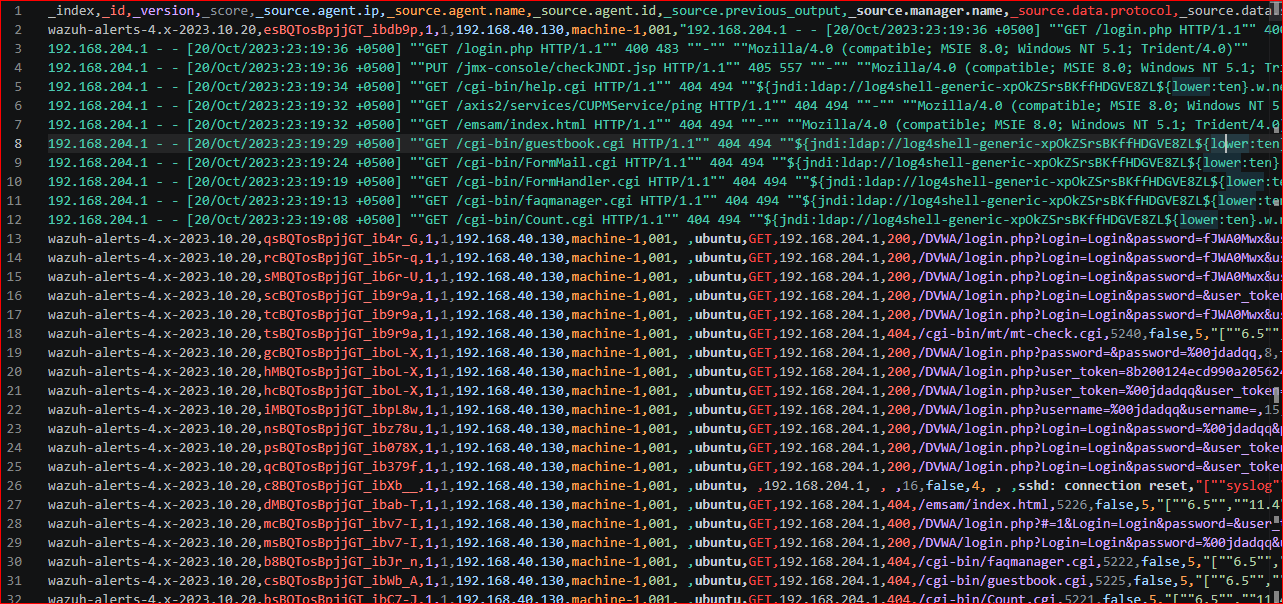
\includegraphics[width=0.7\textwidth]{figures/linux_apt.PNG}
    \caption{Visual representation of the Linux-APT-Dataset-2024}
    \label{fig:linux_apt_data}
\end{figure}

\textbf{Published ML/AI Work:} As of 2025–2026, no independent ML/AI study has yet used this dataset for model training or evaluation beyond the original description paper — a direct consequence of the typical 6–18 month publication cycle. However, related prior work on Linux log-based APT detection provides methodological context: Chen et al. (2020) proposed a detection approach based on Linux logs \cite{chen2020linux}, using log parsing and anomaly analysis to identify advanced attacks, achieving promising results in controlled environments \cite{karim2024linux}. This work illustrates the methodological direction that future studies exploiting Linux-APT-Dataset-2024 are likely to follow.

\subsubsection{MLAPT Dataset}

The MLAPT dataset accompanies the paper \textit{"A Cyber Kill Chain Approach for Detecting Advanced Persistent Threats"} (Ancona et al.), available both at the GitHub repository `APT\_detector/MLAPT\_dataset.csv` and via the Loughborough University repository. This dataset is particularly aligned with our work because it is explicitly structured around the \textbf{Cyber Kill Chain model} — the primary threat modeling framework of this thesis as shown in Figure~\ref{fig:ml_apt_data}. Alerts are labeled according to CKC phases, making it a natural benchmark for evaluating stage-aware APT detection models and a direct validation ground for our proposed sequential detection architecture.

\begin{figure}[H]
    \centering
    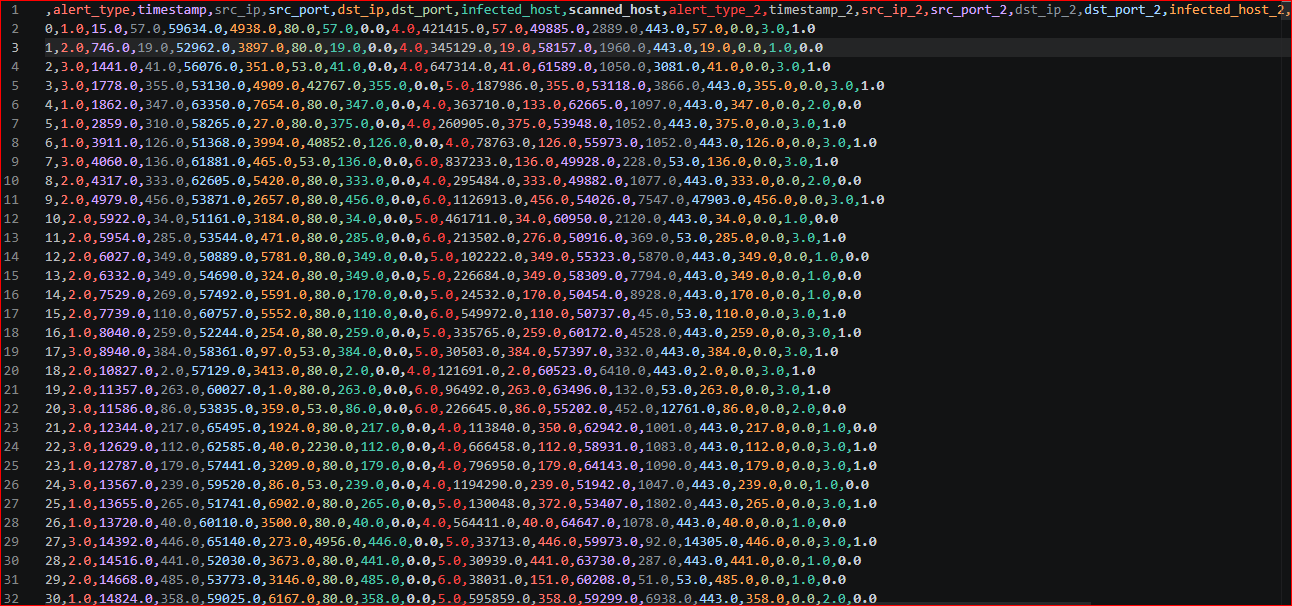
\includegraphics[width=0.7\textwidth]{figures/ml_apt.PNG}
    \caption{Visual representation of the MLAPT dataset}
    \label{fig:ml_apt_data}
\end{figure}

\subsubsection{KAPT-2024}

Tapsoba et al. introduced KAPT-2024 in \textit{"A Relevant Feature Identification Approach to Detect APTs in HTTPS Traffic"} (IJACSA, 2024), generated using the KExtractor tool and hosted on GitHub. The dataset focuses on HTTPS-encrypted traffic — a realistic and challenging scenario since APT actors increasingly use encrypted channels to blend C2 communication into legitimate traffic, further visualized in Figure~\ref{fig:kapt_data}. The paper itself constitutes the primary reference for this dataset and presents a feature identification approach as part of the same publication; no independent research team has yet exploited it.

\begin{figure}[H]
    \centering
    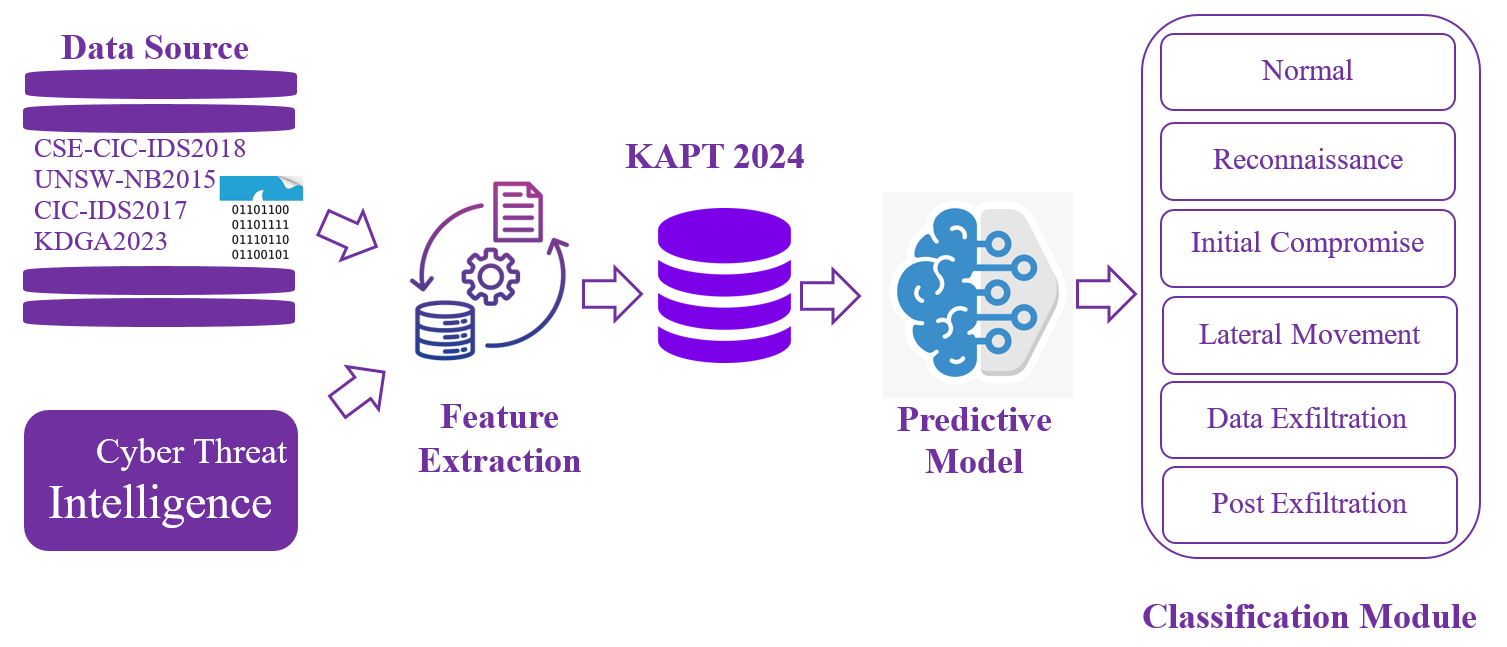
\includegraphics[width=0.7\textwidth]{figures/kapt.png}
    \caption{Visual overview of the KAPT-2024 dataset}
    \label{fig:kapt_data}
\end{figure}

\textbf{Published ML/AI Work:} The originating paper by Tapsoba et al. presents a relevant feature identification pipeline applied to KAPT-2024. In the broader encrypted-traffic detection domain, Yue et al. (2024) proposed \textbf{AISL} (Attack Intent-driven Sequence-based Learning), which integrates heterogeneous audit data and constructs provenance graphs annotated with attack-intent security tags. Evaluated on 10 realistic APT scenarios, AISL achieved a precision of \textbf{93.05\%}, recall of \textbf{98.12\%}, and F1-score of \textbf{95.36\%} [2]. Although AISL does not use KAPT-2024 directly, its methodology — combining provenance graphs with sequential learning — is directly applicable and represents the state-of-the-art for encrypted-channel APT detection.

\subsubsection{Windows APT Persistence Techniques Dataset (2025)}

Riahi and Debatty published this dataset at IEEE ICIN 2025, described as \textit{"Dataset of APT Persistence Techniques on Windows Platforms Mapped to the MITRE ATT\&CK Framework"}, available on Mendeley Data. It provides comprehensive persistence behavior traces mapped to ATT\&CK TA0003 (Persistence), with a focus on tactics employed by Chinese threat actors. The \textbf{Persistence} tactic is one of the defining characteristics of APTs — adversaries maintain long-term, undetected foothold within compromised systems — making this dataset directly relevant to the Installation and C2 phases of the CKC.

\textbf{Published ML/AI Work:} This dataset was published at an IEEE conference in early 2025 and currently has only 2 Scopus citations; no ML/AI study has yet used it independently. However, related prior work is instructive: Matsuda et al. (2018) applied unsupervised anomaly detection to Windows Event logs to detect APT attacks against Active Directory using legitimate administrator accounts, achieving high precision in identifying anomalous authentication patterns [3]. Ling et al. (2023) further surveyed adversarial attacks against Windows PE malware \cite{ling2023windows} detection, demonstrating the critical importance of Windows-specific attack vectors and the robustness challenges any model must address on this platform [4].

\subsubsection{CICAPT-IIoT \cite{ghiasvand2024cicapt}}

Ghiasvand et al. introduced CICAPT-IIoT \cite{ghiasvand2024cicapt} in arXiv preprint 2407.15130 (2024), described as \textit{"CICAPT-IIoT \cite{ghiasvand2024cicapt}: A Provenance-Based APT Attack Dataset for IIoT Environment"}, available via CIC Research Canada and Kaggle. The dataset covers more than 4 GB of IIoT network traffic records integrating 20 MITRE ATT\&CK techniques. Its \textbf{provenance-based} approach records the causal chain of system events (file reads, process forks, network connections) rather than only network flows — enabling graph-based analysis of APT propagation, which is essential for our GNN-based Proposition 2, as depicted in Figure~\ref{fig:cicapt_iot_data}.

\begin{figure}[H]
    \centering
    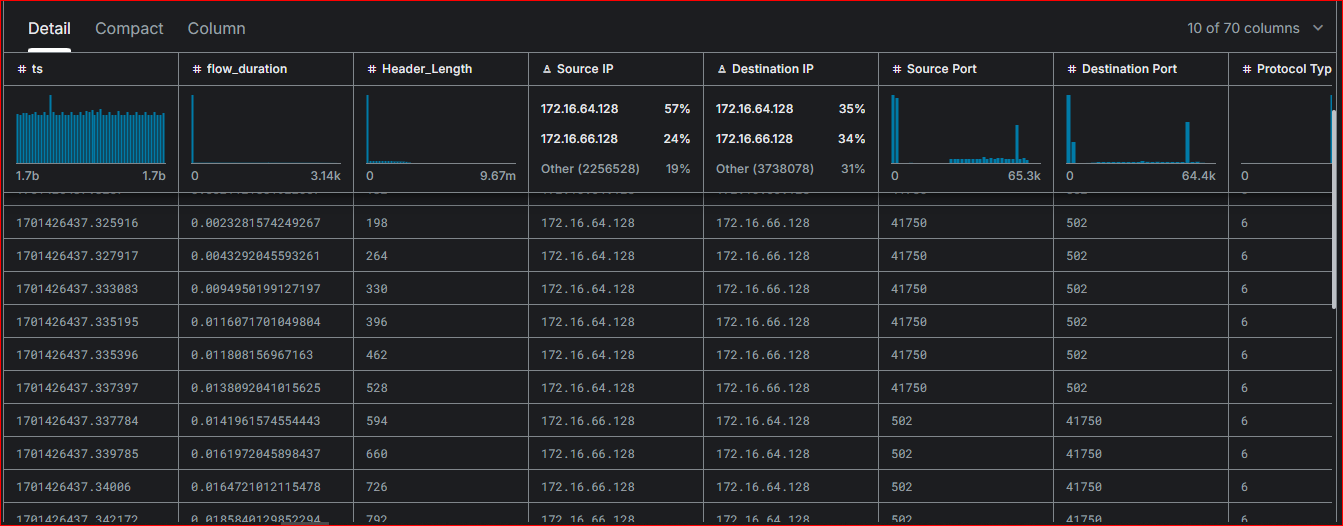
\includegraphics[width=0.7\textwidth]{figures/iot.PNG}
    \caption{Visual overview of the CICAPT-IIoT dataset}
    \label{fig:cicapt_iot_data}
\end{figure}

\textbf{Published ML/AI Work Using CICAPT-IIoT \cite{ghiasvand2024cicapt}:} One important study has directly applied a deep learning model to this dataset. The paper proposes a \textbf{CNN2D-based framework} for IoT cyberattack detection on CICAPT-IIoT \cite{ghiasvand2024cicapt}, following an 8-step pipeline:

\begin{enumerate}
\item Data acquisition from the CICAPT-IIoT \cite{ghiasvand2024cicapt} dataset (attack records + balanced normal subset)
\item Preprocessing: null value handling, Label Encoding, shuffling, normalization
\item Advanced feature engineering: correlation analysis, PCA for dimensionality reduction, temporal windowing
\item Feature scaling: both Min-Max and Z-score normalization tested
\item \textbf{2D reshaping} of feature vectors into matrix format (image-like) to enable CNN2D spatial processing
\item Train/test split
\item Real-time prediction deployment
\end{enumerate}

The CNN2D architecture uses 3 convolutional layers (3×3 and 5×5 kernels), ReLU activation, Max-Pooling, Dropout (rate = 0.3), and Softmax output. Hyperparameters were tuned via grid search + cross-validation (batch size: 128, learning rate: 0.001, optimizer: Adam, loss: categorical cross-entropy).

\textbf{Table 3.3 — CNN2D vs. Baseline Models on CICAPT-IIoT \cite{ghiasvand2024cicapt}}

| Algorithm | Accuracy (\%) | Precision (\%) | Recall (\%) | F1-Score (\%) |
|---|---|---|---|---|
| \textbf{CNN2D (Proposed)} | \textbf{99.78} | \textbf{99.7} | \textbf{99.8} | \textbf{99.75} |
| Logistic Regression | 99.70 | 99.0 | 99.8 | 99.70 |
| Random Forest | 96.00 | 95.2 | 96.5 | 95.80 |
| SVM | 94.00 | 93.4 | 94.1 | 93.70 |

For scalability, the CNN2D model maintained \textbf{99.78\% accuracy on 50,000 records} (avg. prediction time: 1.2 s) and \textbf{99.65\% accuracy on 200,000 records} (avg. prediction time: 3.8 s), confirming strong discriminative capacity even on the highly imbalanced dataset (~95\% normal / ~5\% attack). This result directly validates CICAPT-IIoT \cite{ghiasvand2024cicapt} as a viable training and evaluation benchmark and provides a strong performance reference point for our own experimental phase.

In the broader IIoT-APT detection space, Saurabh et al. (2024) proposed \textbf{HMS-IDS}, a hybrid multi-stage IDS combining supervised and unsupervised approaches for known and zero-day attack detection in IIoT environments (evaluated on CIC-ToN-IoT), achieving \textbf{99.49\% accuracy for known attacks} and \textbf{98.32\% for zero-day attacks} [5]. Gueye et al. (2023) also achieved promising results for Modbus-protocol IoT/IIoT attack detection using deep learning [6].

\subsubsection{MITRE TTP Mapping Datasets (TRAM, Procedure+, Expert)}

This collection is available on HuggingFace and GitHub (tumeteor/Security-TTP-Mapping), associated with articles on Noise Contrastive Estimation-based matching, AnnoCTR entity detection, and LLM-driven CTI generation. The TRAM (Threat Report ATT\&CK Mapper) dataset is a structured collection of CTI reports labeled with MITRE ATT\&CK techniques, used to benchmark NLP and LLM-based TTP extraction. For our GenAI-augmented detection proposition (Section 3.6.2), where we propose LLM-based automated CTI analysis and TTP mapping, these datasets serve as direct evaluation benchmarks.

\subsubsection{APT Audit Logs for 5 Groups}

Available at GitHub (skrghosh/apt-dataset), this dataset contains audit log traces attributed to five distinct APT groups with MITRE ATT\&CK annotations. Multi-group APT datasets are particularly rare because they allow the model to learn group-specific behavioral signatures — critical for attribution tasks and for testing the generalizability of detection models across different adversary profiles.

\subsubsection{LOTL APT Red Team Dataset}

Hosted on Kaggle (cyberprince/lotl-apt-red-team-dataset), this dataset focuses on \textbf{Living-off-the-Land (LOTL)} APT techniques — adversaries using legitimate system tools (PowerShell, WMI, certutil) instead of custom malware. LOTL attacks are among the most challenging to detect because they produce minimal distinctive signatures and blend seamlessly with normal administrative activity. This dataset is essential for evaluating our model's ability to detect technique-level anomalies rather than simple malware signatures.

\subsubsection{CloudAPT Dataset}

Published via the National Research Council of Canada's digital repository, this dataset covers APT attack steps in cloud environments. Cloud-specific APT datasets are currently underrepresented in the community, making this resource particularly valuable as enterprise infrastructure continues its shift to cloud platforms.

\subsubsection{APT Lateral Movement Dataset (LMD Collections)}

Linked to the article \textit{"Enhanced Detection of APT Vector Lateral Movement in Organizational Networks Using Lightweight Machine Learning"} and accessible at GitHub (ChristosSmiliotopoulos/Lateral-Movement-Dataset--LMD\_Collections), with additional collections via Google Drive. \textbf{Lateral movement} (MITRE ATT\&CK TA0008) is one of the most diagnostically significant APT phases, where the adversary pivots between systems to reach high-value targets. A dedicated lateral movement dataset allows fine-grained evaluation of LSTM and GNN components that must correlate events across multiple hosts and time windows.

\subsubsection{APTNotes (Modified Cyber Kill Chain Model)}

Available at GitHub (aptnotes/data), associated with \textit{"Modified Cyber Kill Chain (MCKC): A Cognitive Model for APT Analysis"}. This collection consists of structured threat intelligence reports describing real-world APT campaigns. Unlike raw log datasets, these reports are the natural input for NLP-based TTP extraction — a key component of our GenAI-augmented proposition.

\subsubsection{RBD24 — Risk-Based Labelled Log Dataset}

Hosted on Zenodo (record 13787591), RBD24 provides labeled application log data annotated with risk-based activities. Its risk-score labeling (rather than binary attack/benign) is more aligned with the probabilistic reward shaping in our RL-driven detection framework (Proposition 1).

\subsubsection{APT Persistence Dataset (CyLab)}

Available at GitLab (cylab/datasets/apt-persistence), this dataset complements the Windows APT Persistence dataset by providing a platform-agnostic view of adversarial persistence mechanisms.

\subsubsection{KillChainGraph (MITRE ATT\&CK ↔ CKC Mapping Framework)}

The KillChainGraph project (Frondeur-Labs/KillChainGraph on GitHub) provides a phase-aware multi-model ML framework that maps MITRE ATT\&CK techniques to the seven CKC phases, forming phase-specific labeled sub-datasets. ATTACK-BERT maps techniques to seven phases, and the framework evaluates LightGBM, a custom Transformer, fine-tuned BERT, and GNN with weighted soft-voting ensemble. This directly parallels our proposed architecture and provides a reference implementation for ATT\&CK ↔ CKC phase mapping.

\textbf{Summary Table — Datasets With CKC/MITRE ATT\&CK Mapping}

| Dataset | Mapping | Environment | Key Relevance to Our Work |
|---|---|---|---|
| Linux-APT-Dataset-2024 | MITRE ATT\&CK | Linux | Linux-specific labeled APT logs |
| MLAPT | CKC Phases | Network | CKC-aligned alert labeling |
| KAPT-2024 | MITRE ATT\&CK | HTTPS Traffic | Encrypted C2 detection |
| Windows APT Persistence 2025 | MITRE ATT\&CK | Windows | Persistence tactic (TA0003) |
| CICAPT-IIoT \cite{ghiasvand2024cicapt} | MITRE ATT\&CK | IIoT | Provenance graphs, CNN2D validated |
| TRAM/TTP Mapping | MITRE ATT\&CK | CTI Text | NLP/LLM TTP extraction |
| APT Audit Logs (5 Groups) | MITRE ATT\&CK | Multi-env | Multi-group generalization |
| LOTL APT Red Team | MITRE ATT\&CK | Windows | Living-off-the-land detection |
| CloudAPT | Likely ATT\&CK | Cloud | Cloud-based APT scenarios |
| LMD Collections | Partial ATT\&CK | Network | Lateral movement evaluation |
| APTNotes (MCKC) | CKC (Modified) | CTI Reports | NLP-based TTP extraction |
| RBD24 | Risk-labeled | App Logs | Risk-scored annotation |
| APT Persistence (CyLab) | Partial | Multi-platform | Persistence mechanism study |
| KillChainGraph | ATT\&CK ↔ CKC | Multi | Phase-aware ML benchmarking |

\subsection{Broader Cybersecurity Datasets — Not Directly Suited to Our Work}

The survey by Ankalaki et al. \cite{ankalaki2025cyber} covers an extensive catalog of cybersecurity benchmark datasets across seven categories. While these datasets are widely adopted for evaluating ML/DL models in general intrusion detection, they are \textbf{not directly suited to our APT multi-stage detection objective} for two primary reasons: (1) they lack MITRE ATT\&CK or CKC annotations that would allow stage-aware evaluation, and (2) most capture isolated, single-stage attack events rather than the temporally correlated, multi-phase sequences that define APT campaigns. They nonetheless form the foundational literature landscape from which our work departs.

\subsubsection{Network Traffic-Based Datasets}

As documented in \cite{ankalaki2025cyber}, this is the most studied category in intrusion detection research:

\begin{itemize}
\item \textbf{KDD Cup 1999 / NSL-KDD}: Historically the most cited IDS datasets, containing four attack categories (DoS, U2R, R2L, Probe). Widely criticized for outdated traffic patterns, redundant data, and unrealistic scenarios that do not reflect modern APT techniques \cite{ankalaki2025cyber}.
\item \textbf{UNSW-NB15 (2015)}: Ten attack categories including backdoors and shellcode, generated over 31 hours of emulated traffic. More diverse than KDD, but attacks remain isolated events rather than multi-stage campaigns \cite{ankalaki2025cyber}.
\item \textbf{CICIDS2017}: One of the most comprehensive modern IDS datasets — 3.1M flows, 8 attack types (SQL injection, DoS, DDoS, botnet, brute force, etc.) over 5 days. Despite its richness, it lacks APT-specific attack chains or CKC/ATT\&CK annotations \cite{ankalaki2025cyber}.
\item \textbf{LITNET 2020}: Recent dataset with 12 attack types from real network traffic, small in size and focused on known cataloged signatures \cite{ankalaki2025cyber}.
\item \textbf{HIKARI-2021}: Covers bruteforce variants and cryptomining over 39 hours of real traffic \cite{ankalaki2025cyber}.
\end{itemize}

The fundamental limitation of this entire category for our purposes is that they capture \textit{what happened} (attack type), not \textit{where in the attack lifecycle it happened} (kill chain phase).

\subsubsection{Malware and Android-Based Datasets}

\begin{itemize}
\item \textbf{CIC-AndMal2017 / CCCS-CIC-AndMal-2020}: Android malware datasets covering spyware, trojans, adware, ransomware. Useful for endpoint-level malware classification (CKC Phase 2 — Weaponization) but provide no multi-stage campaign context.
\item \textbf{SoReL-20M}: Over 20 million malware samples. Impressive scale for malware classification but no temporal or campaign-level APT structure.
\end{itemize}

\subsubsection{IoT Traffic-Based Datasets}

\begin{itemize}
\item \textbf{TON-IoT (2020)}: Nine attack types in IoT environments, simulated traffic. LSTM achieved 97\% accuracy and CNN 99\% \cite{ankalaki2025cyber}. However, attacks are individually labeled without CKC phase structure.
\item \textbf{Bot-IoT (2019)}: 46-feature botnet detection dataset where LSTM achieved ~98\% and SVM ~99\% \cite{ankalaki2025cyber}. No CKC/ATT\&CK phase annotations.
\item \textbf{X-IIoTID (2021)}: 18 attack types including reconnaissance, lateral movement, and C2 — features partially overlapping with CKC phases. GRU achieved 99.46\% accuracy \cite{ankalaki2025cyber}. Its lack of explicit CKC mapping limits its use for stage-aware evaluation, though it is the closest in this category to APT-relevant data.
\end{itemize}

\subsubsection{APT-Specific Datasets Without Explicit Mapping}

\begin{itemize}
\item \textbf{DAPT 2020 \cite{myneni2020dapt}}: Purpose-built for APT detection (\textit{"DAPT 2020 \cite{myneni2020dapt} - Constructing a Benchmark Dataset for Advanced Persistent Threats"}, Kaggle). Its annotation scheme does not follow the MITRE ATT\&CK taxonomy, limiting ATT\&CK-coverage evaluation.
\item \textbf{Unraveled \cite{myneni2023unraveled} APT Dataset}: A semi-synthetic dataset for APT research (Kaggle). Semi-synthetic nature means some behaviors may not faithfully represent real-world APT tradecraft.
\item \textbf{LANL Multi-Source Cybersecurity Events}: Real-world dataset from Los Alamos National Laboratory containing 90 days of anonymized internal network events (authentication logs, process events, DNS queries). Highly realistic and temporally rich, associated with an RNN attention mechanism paper (arXiv:1803.04967), but lacks APT-specific labels and CKC annotations.
\item \textbf{CIC-IDS2018}: Available on Kaggle and AWS; used in APT-adjacent studies but focused on individual attack types rather than multi-stage campaigns.
\end{itemize}

\subsubsection{Systemic Limitations for APT Stage-Aware Detection}

The review of datasets in Ankalaki et al. \cite{ankalaki2025cyber} reveals several systemic limitations when applied to the APT detection problem:

\begin{enumerate}
\item \textbf{Narrow Attack Scope}: Datasets like MQTT-IoT-IDS2020 provide few attack classes, restricting model generalizability to the wide variety of real-world APT techniques.
\item \textbf{Outdated or Simulated Traffic}: Older datasets (Bot-IoT 2019) do not capture modern APT techniques; simulation-based datasets (TON-IoT) fail to reproduce the complexity of real-world APT campaigns.
\item \textbf{Absence of Stage Annotations}: The most critical limitation — none of the general benchmark datasets in \cite{ankalaki2025cyber} provide kill-chain phase or ATT\&CK technique annotations, making them unsuitable for evaluating the stage-aware component of our framework.
\item \textbf{Class Imbalance}: APT-related traffic constitutes a minuscule fraction of total network activity, as confirmed by CICAPT-IIoT \cite{ghiasvand2024cicapt}'s ~95\%/5\% normal-to-attack ratio.
\item \textbf{Lack of Provenance Context}: Standard flow-based datasets discard causal relationships between events (which process spawned which network connection), essential for graph-based APT detection.
\end{enumerate}

\subsection{Review of AI/ML Works on APT Datasets — Methods and Results}

Beyond the CNN2D result on CICAPT-IIoT \cite{ghiasvand2024cicapt} (Section 3.4.1.5), the following works represent the state-of-the-art in AI/ML-based APT detection using datasets comparable to those in our work:

\textbf{Bodström \& Hämäläinen (2019) — Novel Deep Learning Stack for APT Detection [7]}  
Proposed a multi-layer deep learning architecture combining different DL methods adapted for APT detection using raw network flows. This work is one of the first to specifically target APT-level threats with a pure DL stack, establishing important architectural baselines for subsequent research.

\textbf{Matsuda et al. (2018) — APT Detection Against Active Directory [3]}  
Applied unsupervised anomaly detection (machine learning on Windows Event Logs) to detect APT attacks using legitimate administrator accounts. Achieved high precision in identifying anomalous authentication sequences on Windows environments — directly relevant to the Windows APT Persistence Techniques Dataset context.

\textbf{Yue et al. (2024) — AISL: Attack Intent-driven Sequence-based Learning [2]}  
Constructed provenance graphs from heterogeneous audit logs and assigned security tags based on attack intent. A sequential learning model then detects APT stages from graph event sequences. Evaluated on 10 realistic APT scenarios: \textbf{Precision: 93.05\%, Recall: 98.12\%, F1: 95.36\%}. Particularly notable for its high recall, which is the priority metric in APT detection.

\textbf{Saurabh et al. (2024) — HMS-IDS for IIoT [5]}  
Hybrid multi-stage IDS combining supervised (for known attacks) and unsupervised (for zero-day) approaches, integrating threat intelligence. Evaluated on CIC-ToN-IoT: \textbf{99.49\% accuracy for known attacks, 98.32\% for zero-day attacks}. Demonstrates the viability of hybrid detection in IIoT environments directly adjacent to the CICAPT-IIoT \cite{ghiasvand2024cicapt} context.

\textbf{Layeghy \& Portmann (2023) — Cross-Domain Evaluation of ML-based NIDS [8]}  
Studied the transferability of ML intrusion detection models across different datasets. The key finding is that models trained on one dataset often perform significantly worse when applied to another — a critical limitation that justifies dataset diversity in our experimental design and motivates our synthetic data generation component (ReALTabFormer).

\textbf{Stojanović et al. (2020) — APT Datasets and Attack Modeling Review [9]}  
A comprehensive review of APT datasets and modeling for automated detection methods. The study identified a critical shortage of realistic, standardized APT datasets — a finding that directly motivates our use of multiple specialized datasets (MLAPT, KAPT-2024, CICAPT-IIoT \cite{ghiasvand2024cicapt}) and our GenAI-based synthetic scenario generation.

\textbf{Summary Table — AI/ML Works on APT-Relevant Datasets}

| Reference | Method | Dataset | Key Results |
|---|---|---|---|
| CNN2D Paper (2024) | CNN2D + PCA + grid search | CICAPT-IIoT \cite{ghiasvand2024cicapt} | Acc. 99.78\%, F1 99.75\% |
| Yue et al. [2] (2024) | Provenance graph + AISL | Heterogeneous APT logs | Prec. 93.05\%, Rec. 98.12\%, F1 95.36\% |
| Saurabh et al. [5] (2024) | HMS-IDS (Hybrid) | CIC-ToN-IoT | 99.49\% known, 98.32\% zero-day |
| Bodström \& Hämäläinen [7] (2019) | Deep Learning Stack | Network flows | APT-specific DL baseline |
| Matsuda et al. [3] (2018) | Unsupervised anomaly detection | Windows Event Logs | High precision AD-APT detection |
| Layeghy \& Portmann [8] (2023) | Cross-domain ML evaluation | Multi-dataset | Poor cross-dataset transferability |

\subsection{Dataset Selection Rationale for Our Experimental Phase}

The landscape of APT detection datasets is fragmented: the most realistic datasets (LANL, CICIDS2017) lack ATT\&CK annotations, while the most specifically annotated datasets (MLAPT, KAPT-2024, Windows Persistence 2025) are limited in scale or scope. This fragmentation is itself a key motivation for our GenAI-based synthetic data generation component (ReALTabFormer in Proposition 1), which addresses the scarcity of labeled multi-stage APT data.

For the experimental phase of this work, our dataset selection will prioritize:
\begin{itemize}
\item \textbf{MLAPT} and \textbf{Linux-APT-Dataset-2024} as primary training datasets due to their direct CKC and ATT\&CK alignment.
\item \textbf{CICAPT-IIoT \cite{ghiasvand2024cicapt}} for evaluating the GNN-based pre-attack detection framework (Proposition 2) due to its provenance-based structure, scale, and the CNN2D benchmark (99.78\%) as a reference point.
\item \textbf{KAPT-2024} for testing detection under realistic encrypted-traffic scenarios.
\item \textbf{KillChainGraph phase-specific sub-datasets} for benchmarking the ATT\&CK-to-CKC phase mapping component.
\item \textbf{APT Audit Logs (5 Groups)} and \textbf{LOTL APT Red Team Dataset} for cross-group generalization evaluation.
\end{itemize}

---

\section{Synthesis}

A comparative analysis of the described solutions reveals distinct trade-offs between interpretability, accuracy, and computational efficiency.

\textbf{Table 3.4 — Synthesis of Detection Approaches based on \cite{ankalaki2025cyber}}

| Approach | Key Advantages | Limitations |
|---|---|---|
| Traditional ML | High interpretability (DT/RF), low computational overhead, effective for signature-based threats | High false positive rates on complex data; requires extensive feature engineering; fails against obfuscated APTs |
| Deep Learning | Automatic feature extraction; excellent performance on unstructured data; captures temporal dependencies (LSTM) | "Black-box" nature (low interpretability); requires massive labeled datasets which are rare for APTs; high training time |
| Generative AI | Detects zero-day anomalies; handles uncertainty (VAE); generates synthetic training data to balance datasets | Computationally intensive; complex hyperparameter tuning; risk of "hallucinations" in generation tasks |

\textbf{Conclusion of Synthesis:} While Traditional ML provides a baseline, it is insufficient for the stealthy nature of APTs. Deep Learning improves detection capabilities but suffers from opacity and data scarcity. Generative AI addresses the data scarcity and anomaly detection capabilities but requires careful integration. Currently, a gap exists in the literature: most solutions are reactive classifiers. There is a critical need for a framework that not only detects (Perception) but also decides on the optimal response strategy (Decision-Making) while handling the multi-stage nature of APTs mapped to the Cyber Kill Chain.

---

\section{Proposition}

To address the limitations identified in the synthesis — specifically the lack of proactive decision-making and the challenge of multi-stage correlation — this thesis proposes a dual-framework architecture. This architecture integrates Generative AI for enhanced perception and synthetic data generation, with Reinforcement Learning for optimal defense strategy.

\subsection{Proposition 1: RL-Driven Decision-Making Framework}

Our first proposition introduces a \textbf{Reinforcement Learning-driven decision-making framework} designed for early defense against multi-stage APT attacks, explicitly mapped to the Cyber Kill Chain to ensure stage-aware mitigation.

\textbf{Architecture Overview}

The core innovation of this proposition is the decoupling of Perception (interpreting the environment) from Decision-Making (taking action). This separation allows for more modular and robust training.

\textbf{The Multi-Model Perception Layer}

Instead of relying on a single detection algorithm, the framework employs a composite perception module consisting of three specialized pre-trained models:

\begin{enumerate}
\item \textbf{Autoencoder (AE) for Anomaly Detection:} The AE is trained to minimize the reconstruction error of benign traffic. It acts as the first filter, identifying raw deviations from the baseline.
\item \textbf{Variational Autoencoder (VAE) for Maliciousness Estimation:} The VAE goes beyond simple error reconstruction. It provides a probabilistic estimate of "maliciousness" accompanied by an uncertainty metric. This uncertainty quantification is crucial for reducing false positives in ambiguous scenarios.
\item \textbf{Transformer for State Prediction:} A Transformer model processes the sequence of alerts to predict the likely next stage of the attack in the Cyber Kill Chain. This predictive capability allows the system to be proactive rather than reactive.
\end{enumerate}

These three models work in concert to summarize high-volume alerts into a compact, numerical state representation vector \(S\_t\).

\textbf{The Deep Q-Network (DQN) Agent}

The state vector \(S\_t\) is fed into a custom APT environment where a Deep Q-Network (DQN) agent operates. The agent aims to learn an optimal policy \(\pi(S\_t)\) that maximizes the cumulative reward:

\[Q(s, a) = r + \gamma \max\_{a'} Q(s', a')\]

The agent learns when and how to respond to evolving attacks. The reward function is designed to prioritize early intervention (stopping the attack in the Reconnaissance or Weaponization phase) while heavily penalizing false alarms that disrupt legitimate operations.

\textbf{Training with ReALTabFormer and Conditional Replay}

A major hurdle in training RL agents for cybersecurity is the scarcity of realistic attack traces. We address this by using \textbf{ReALTabFormer}, a generative model tailored for tabular data.

\begin{itemize}
\item \textbf{Synthetic Data Generation:} ReALTabFormer generates diverse, high-level malicious alert attributes based on limited real-world samples.
\item \textbf{Conditional Replay:} To ensure these synthetic attributes are compatible with our perception models, they are mapped back to realistic feature vectors via a conditional replay mechanism.
\end{itemize}

This pipeline enables the agent to train on diverse, realistic attack scenarios — ranging from stealthy low-and-slow attacks to aggressive intrusions — without the need to retrain the underlying detection models.

\subsection{Proposition 2: GenAI-Augmented Pre-Attack Detection Framework}

Complementing the decision-making framework, our second proposition focuses on the structural detection of APTs using a \textbf{GenAI-Augmented Pre-Attack Detection Framework}. This approach leverages the structural nature of network data to identify pre-attack behaviors.

\textbf{Unified Cyber Kill Chain Mapping}

To cover the full spectrum of APT activities, we propose a mapping scheme that integrates the conventional Cyber Kill Chain (CKC) with the MITRE ATT\&CK framework. This unified chain provides a granular view of adversary TTPs, spanning from initial reconnaissance to the final impact.

\textbf{Graph-Based Representation and GNNs}

Network entities (hosts, users, files, IP addresses) and their interactions are modeled as a heterogeneous graph \(G = (V, E)\).

\begin{itemize}
\item \textbf{Graph Neural Networks (GNN):} We employ GNNs to analyze this graph structure. GNNs are capable of learning node embeddings that capture the neighborhood context.
\item \textbf{Pre-Attack Detection:} The GNN is trained to identify sub-graph patterns indicative of pre-attack activities (e.g., scanning, enumeration) which appear as specific topological structures within the network graph, often invisible to flow-based detectors.
\end{itemize}

\textbf{GenAI for Synthetic Scenario Generation}

Validating APT detection models is challenging due to the lack of public datasets containing multi-stage attacks. We utilize Generative AI to create synthetic APT scenarios:

\begin{itemize}
\item \textbf{Scenario Generation:} GenAI models generate synthetic sequences of MITRE ATT\&CK techniques that mimic the logic and progression of real APT groups (e.g., APT29, APT41).
\item \textbf{Integration:} These synthetic scenarios are injected into the training pipeline, ensuring the GNN model is robust against unseen attack vectors.
\end{itemize}

\textbf{Cyber Threat Intelligence (CTI) Platform Integration}

To operationalize this framework, we propose its integration into a CTI platform built on the ELK stack (Elasticsearch, Logstash, Kibana):

\begin{enumerate}
\item \textbf{Data Ingestion:} Logstash collects logs from various sources (syslogs, firewall, IDS).
\item \textbf{Processing:} The GenAI-Augmented GNN models analyze incoming data streams in real-time.
\item \textbf{Visualization:} Kibana provides a dashboard for security analysts, visualizing the predicted attack stages and the graph-based alerts, facilitating rapid incident response.
\end{enumerate}

---

\section{Chapter Conclusion}

In this chapter, we reviewed the spectrum of APT detection solutions, highlighted the progression from traditional ML to Generative AI, and conducted a comprehensive study of the existing APT datasets landscape. We identified that while GenAI offers powerful capabilities for anomaly detection and data synthesis, it requires a robust decision-making layer to be operationally effective. The dataset study revealed that the four most relevant recent datasets (Linux-APT-Dataset-2024, KAPT-2024, Windows APT Persistence 2025, CICAPT-IIoT \cite{ghiasvand2024cicapt}) are newly published resources with no independent ML/AI studies yet — confirming that our work has the opportunity to produce among the first experimental results on these benchmarks. The CNN2D study on CICAPT-IIoT \cite{ghiasvand2024cicapt} (99.78\% accuracy) establishes an important performance reference, while cross-domain evaluation results from Layeghy \& Portmann [8] motivate our multi-dataset experimental strategy and synthetic data generation component.

Our proposed solution is twofold: (1) An RL-driven framework utilizing a multi-model perception layer (AE, VAE, Transformer) and synthetic training data (ReALTabFormer) to automate defense strategies; and (2) A GenAI-Augmented GNN framework integrated into a CTI platform for the structural detection of pre-attack behaviors. Together, these propositions aim to significantly reduce the dwell time of APTs and enhance the resilience of critical systems.

---

\#\# References

\cite{karim2024linux} L. Chen et al., "Detecting Advanced Attacks Based On Linux Logs \cite{chen2020linux}," in \textit{2020 IEEE 6th Intl Conference on Big Data Security on Cloud (BigDataSecurity)}, IEEE, May 2020, pp. 60–64. doi: 10.1109/bigdatasecurity-hpsc-ids49724.2020.00022.

[2] H. Yue, T. Li, D. Wu, R. Zhang, and Z. Yang, "Detecting APT attacks using an attack intent-driven and sequence-based learning approach," \textit{Computers \& Security}, vol. 140, p. 103748, May 2024. doi: 10.1016/j.cose.2024.103748.

[3] W. Matsuda, M. Fujimoto, and T. Mitsunaga, "Detecting APT Attacks Against Active Directory Using Machine Learning," in \textit{2018 IEEE Conference on Application, Information and Network Security (AINS)}, IEEE, Nov. 2018, pp. 60–65. doi: 10.1109/ains.2018.8631486.

[4] X. Ling et al., "Adversarial attacks against Windows PE malware \cite{ling2023windows} detection: A survey of the state-of-the-art," \textit{Computers \& Security}, vol. 128, p. 103134, May 2023. doi: 10.1016/j.cose.2023.103134.

[5] K. Saurabh, V. Sharma, U. Singh, R. Khondoker, R. Vyas, and O. P. Vyas, "HMS-IDS: Threat Intelligence Integration for Zero-Day Exploits and Advanced Persistent Threats in IIoT," \textit{Arabian Journal for Science and Engineering}, vol. 50, no. 2, pp. 1307–1327, Jul. 2024. doi: 10.1007/s13369-024-08935-5.

[6] T. Gueye, Y. Wang, M. Rehman, R. T. Mushtaq, and S. Zahoor, "A novel method to detect cyber-attacks in IoT/IIoT devices on the modbus protocol using deep learning," \textit{Cluster Computing}, vol. 26, no. 5, pp. 2947–2973, Jun. 2023. doi: 10.1007/s10586-023-04028-4.

[7] T. Bodström and T. Hämäläinen, "A Novel Deep Learning Stack for APT Detection," \textit{Applied Sciences}, vol. 9, no. 6, p. 1055, Mar. 2019. doi: 10.3390/app9061055.

[8] S. Layeghy and M. Portmann, "Explainable Cross-domain Evaluation of ML-based Network Intrusion Detection Systems," \textit{Computers and Electrical Engineering}, vol. 108, p. 108692, May 2023. doi: 10.1016/j.compeleceng.2023.108692.

[9] B. Stojanović, K. Hofer-Schmitz, and U. Kleb, "APT datasets and attack modeling for automated detection methods: A review," \textit{Computers \& Security}, vol. 92, p. 101734, May 2020. doi: 10.1016/j.cose.2020.101734.
